    \section{Aufbau}
        In \autoref{fig:Aufbau} ist der Versuchsaufbau zu sehen.
        P1 beschreibt die Drehschieberpumpe, P2 die Turbomolekularpumpe.
        V1 und V2 zeigen auf die Ventile der entsprechenden Pumpen, mit diesen Ventilen können die Pumpen abgeschoben werden.
        Zum Einstellen des Gleichgewichtsdruck dienen die Ventile V3 und das Dosierventil D, welche unter dem Rezipienten zu finden sind.
        Das Piezo-Pirani-Vakuummeter Typ TPG202 der Firma Pfeiffer Vacuum steht bei M1.
        Weiterhin gibt es zwei Kaltkathoden-Vakuummeter M2 und M3, es handelt sich um den Typ PKR 360 von Pfeiffer Vacuum, welche jeweils mit einem Anzeigegerät TPG 361 
        von Pfeiffer Vacuum verbunden sind.
        Eins ist dabei an der Turbomolekularpumpe angeschlosssen, das andere hinter dem Dosierventil.

        \begin{figure}[H]
            \centering
            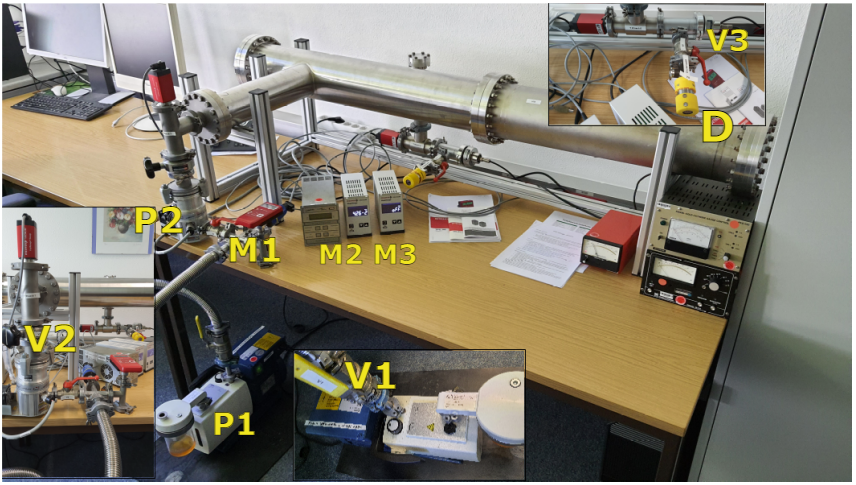
\includegraphics[width=\textwidth]{bilder/Aufbau.png}
            \caption{Der Versuchsaufbau \cite{anleitung}.}
            \label{fig:Aufbau}
        \end{figure}

    \section{Durchführung}
    \label{sec:Durchführung}
        Während des Kolloquiums wird die Drehschieberpumpe gestartet.
        Dabei wird darauf geachtet, welcher Druck erreicht werden kann und somit wird auch überprüft ob die Anlage dicht und funktionsfähig ist.
        % Es bildet sich ein Endruck von $\SI{3.85e-3}{\milli\bar}$.
        Daraufhin kann die Turbomolekularpumpe angeschaltet werden.
        Ebenfalls wird geprüft, wie klein der Druck wird um den Aufbau zu prüfen.
        % Der Endruck hier beträgt $\SI{1.09e-5}{\milli\bar}$.

        \subsection{Turbomolekularpumpe}
            Bei der Turbomolekularpumpe handelt es sich um das Modell Turbo SST81 von der Firma ILMVAC und wird mit $\SI{1350}{\hertz}$ betrieben.
            Laut Hersteller beträgt das Saugvermögen $\SI{77}{\litre\per\second}$ \cite{anleitung}.

            \subsubsection{Leckratenmessung}
                Zunächst wird eine Leckratenmessung durchgeführt.
                Mithilfe des gelben Dosierventils wird ein konstanter Gleichgewichtsdruck im Rezipienten eingestellt.
                Dabei ist das Ventil zur Turbomolekularpumpe geöffnet.
                Nun wird das Ventil verschlossen und die Messung wird gestartet, indem der Druck alle $\SI{10}{\second}$ aufgenommen wird.
                Dieser Messvorgang wird insgesamt drei Mal wiederholt für vier verschiedenen Leckraten.
                Ein Messvorgang beträgt dabei $\SI{120}{\second}$.
                Die Gleichgewichtsdrücke betragen $\SI{2e-4}{\milli\bar}, \, \SI{1e-4}{\milli\bar}, \, \SI{7e-5}{\milli\bar}$ und $\SI{5e-5}{\milli\bar}$.
                Zur Aufnahme der Messung wurde das Messgerät M2 verwendet.

            \subsubsection{Evakuierungskurve}
                Der Rezipient wird über das gelbe Dosierventil bis zu einem Anfangsdruck von $\SI{5e-3}{\milli\bar}$ belüftet.
                Dann wird das Ventil schnell geschlossen und die Messung gestartet.
                Hier wird der Druck zu Beginn (bis $t \approx \SI{40}{\second}$) alle $\SI{5}{\second}$ aufgenommen, danach nur noch alle $\SI{10}{\second}$, sodass eine Messung $\SI{120}{\second}$ dauert.
                Dieser Messvorgang wird insgesamt drei Mal durchlaufen.
                Dabei werden die Messwerte mit dem Messgerät M2 aufgenommen.

        \subsection{Drehschieberpumpe}
            Die Messungen zur Drehschieberpumpe laufen analog zu der Messung mit der Turbomolekularpumpe ab.
            Die verwendete Drehschieberpumpe ist ebenfalls von der Firma ILMVAC mit dem Typ 300883/AKD16.
            Laut Hersteller beträgt das Saugvermögen $4,6$ bis $\SI{5.5}{\metre\cubic\per\hour}$ und der angegebene Enddruck beträgt $\SI{2e-3}{\milli\bar}$ \cite{anleitung}.

            \subsubsection{Leckratenmessung}
                Analog wird ein Gleichgewichtsdruck mithilfe des gelben Dosierventils eingestellt und danach die Drehschieberpumpe mit dem Ventil direkt über der Pumpe abgeschiebert.
                Der Druck sollte alle $\SI{10}{\second}$ mit dem Messgerät M1 aufgenommen werden, wird in diesem Versuch versehentlich mit M2 aufgenommen, die Messzeit insgesamt beträgt $\SI{200}{\second}$.
                Die Messung wird für vier verschiedene Gleichgewichtsdrücke jeweils drei Mal durchgeführt.
                Die verwendeten Gleichgewichtsdrücke sind $\SI{100}{\milli\bar},\, \SI{50}{\milli\bar},\, \SI{10}{\milli\bar}$ und $\SI{0.5}{\milli\bar}$.
            \subsubsection{Evakuierungskurve}
                Der Rezipient wird bei laufender Drehschieberpumpe über das gelbe Dosierventil belüftet, sodass ein Anfangsdruck von $\SI{1000}{\milli\bar}$ entsteht.
                Das Ventil wird geschlossen und die Messung gestartet. Es wird mit dem Messgerät M2 gemessen.
                Der Druck wird dann alle $\SI{10}{\second}$ aufgenommen, insgesamt für $\SI{600}{\second}$.
                Dieser Messvorgang wird insgesamt drei Mal durchgeführt.
                Dabei werden die Messwerte versehentlich mit dem Messgerät M2 statt mit M1 aufgenommen.